\documentclass[12pt,a4paper]{report}

\usepackage[utf8]{inputenc}
\usepackage[T1]{fontenc}
\usepackage[spanish, es-noshorthands]{babel}
\usepackage{graphicx}
\usepackage{amsmath, amssymb}
\usepackage{geometry}
\usepackage{url}
\usepackage{hyperref}
\usepackage{booktabs}
\usepackage{float}
\usepackage{setspace}
\usepackage{csquotes}
\usepackage[style=apa,backend=biber,sortcites=true,language=spanish]{biblatex}

\addbibresource{referencias.bib}

\geometry{
    left=2.5cm,
    right=2.5cm,
    top=2.5cm,
    bottom=2.5cm
}

\graphicspath{{figuras/}{figuras/clasificador/}{figuras/semantico/}{figuras/integracion/}}

\hypersetup{
    colorlinks=true,
    linkcolor=black,
    urlcolor=blue,
    citecolor=black
}

\title{Prototipo de sistema de traducción de Lengua de Señas Argentina con procesamiento en tiempo pseudo-real}
\author{Maite Nigro \\ Francisco Veron \\ \vspace{0.5cm} \small Director: Esp.\ Ing.\ Gonzalo Avalos Ribas \\ \vspace{0.5cm} \small Co-director: Ing.\ Bruno Constanzo \\ \vspace{1cm} \small Universidad Nacional de Mar del Plata \\ Facultad de Ingeniería \\ Departamento de Ingeniería en Informática}
\date{Agosto 2026}

\begin{document}

\maketitle

\chapter*{Agradecimientos}
De Maite: Para la Flaqui.\\
De Francisco: Para el Diego y Baco.\\
A Miriam Rolls, por su orientación sobre la LSA y la validación del vocabulario del conjunto de datos.

\tableofcontents

\chapter*{Resumen}
En la actualidad, la interacción virtual entre personas sordas y oyentes se limita casi exclusivamente a la comunicación escrita, lo que impide una conversación simétrica en videollamadas. Este Trabajo Final de Grado desarrolla un prototipo de traducción entre la Lengua de Señas Argentina (LSA) y el español oral con procesamiento local en el dispositivo del usuario. El producto entregado es una aplicación de escritorio que captura video desde una cámara web, reconoce 100 glosas de LSA en tiempo pseudo-real, acumula enunciados mediante reglas de segmentación y los traduce a español rioplatense con un modelo de lenguaje ajustado por fine tunning; la salida se muestra en pantalla y/o se sintetiza en voz. El objetivo general fue reducir la asimetría comunicacional en escenarios de emergencia o escasa comunicacion, con un vocabulario de 100 señas validadas por una experta. La metodología combinó desarrollo iterativo, construcción de un corpus propio de LSA y validación empírica por módulos. El clasificador desplegado alcanza 96,48\,\% de exactitud top-1 en validación fuera de línea sobre 91 clases. El traductor semántico (Qwen2.5-3B-Instruct con LoRA) obtiene un Token F1 promedio de 0,50 y ROUGE-L de 0,49 en una reserva de evaluación de 20 pares. El procesamiento de video, la clasificación y la traducción se ejecutan en la computadora del usuario, sin enviar flujos crudos a la nube. Las conclusiones indican viabilidad del enfoque basado en puntos de referencia corporales y modelos compactos, aunque persisten limitaciones de generalización frente a la cámara, validación con usuarios sordos y componentes pendientes (avatar, extensión de navegador y captura del turno del oyente).

\chapter*{Palabras clave:}
Lengua de señas Argentina(LSA), reconocimiento de gestos, \textit{edge computing}, accesibilidad

\chapter{Introducción}
\section{Contexto}
Tradicionalmente, la sociedad abordó a la comunidad sorda desde una perspectiva clínica centrada en la rehabilitación. Ese enfoque omite que la comunidad sorda se identifica, ante todo, como una minoría lingüística con lengua, cultura y gramática propias, independientes del español oral. En la Argentina, la LSA cuenta con reconocimiento legal desde la Ley 27.710 \parencite{argentina2020ley27710}.

En el ámbito digital, las videollamadas son centrales en la vida cotidiana y en la atención de situaciones críticas. Sin embargo, las plataformas actuales no ofrecen una arquitectura bilingüe integrada que admita la LSA como flujo de datos válido en tiempo pseudo-real. Los recursos disponibles suelen limitarse a diccionarios estáticos o repositorios de video, sin capacidad de interpretación automática en contexto conversacional \parencite{inju2024diccionario}.

\section{Motivación}
Este proyecto nace de la necesidad de devolver autonomía a las personas sordas en interacciones cotidianas y sensibles. Resulta fundamental pasar de un paradigma de asistencia a uno de integración lingüística, en el que la tecnología actúe como puente transparente. La posibilidad de reducir la dependencia de intérpretes humanos en situaciones de urgencia o imposibilidad económica, y de garantizar privacidad en diálogos sensibles impulsa una solución basada en inteligencia artificial con procesamiento local (\textit{edge computing}).

\section{Problemática}
La problemática central es la barrera comunicacional que impide una interacción autónoma en entornos digitales. Hoy no existen herramientas locales que traduzcan, en tiempo pseudo-real, el español hablado y la LSA dentro de un vocabulario acotado y validado.

Esa brecha genera exclusión social: las personas sordas dependen de intérpretes o del texto escrito, que para muchas constituye una segunda lengua o directamente no son alfabetizados. Además, los modelos internacionales de reconocimiento de señas están sesgados hacia la Lengua de Señas Americana (ASL), lo que hace indispensable un (\textit{dataset}) y un entrenamiento específicos para la LSA.

\section{Alcance y limitaciones}
El producto desarrollado traduce LSA a texto y/o voz para el oyente, e incorpora un avatar animado para la devolución de mensajes en LSA y una extensión de navegador (no publicada) para aplicaciones de videoconferencias. El sistema comprende reconocimiento gestual, traducción semántica y síntesis local.
No se busca una interpretación de propósito general para conversaciones extensas. El alcance léxico es de 100 señas, validadas por expertos en LSA; seleccionadas para facilitar la recolección de información clave en situaciones de emergencias.

\chapter{Objetivos}
\section{Objetivo general}
Desarrollar un prototipo de traducción de LSA a español rioplatense en tiempo pseudo-real y viceversa, pensado para operar en plataformas de videoconferencia, con el fin de mitigar la asimetría comunicacional y favorecer la autonomía de las personas sordas al interactuar con oyentes no señantes.

\section{Objetivos específicos}
\begin{itemize}
    \item Implementar un clasificador local basado en puntos de referencia corporales para reconocer palabras de LSA.
    \item Integrar un módulo de traducción semántico bidireccional que transforme secuencias de glosas en oraciones coherentes en español rioplatense y, a su vez, convierta oraciones en español rioplatense a señas de la LSA.
    \item Diseñar mecanismos de segmentación conversacional (acumulación de glosas, memoria de contexto y políticas de repetición).
    \item Garantizar privacidad mediante procesamiento exclusivo en el dispositivo.
    \item Desarrollar la arquitectura de la extensión de navegador para videoconferencias, dejándola funcional y lista para su eventual publicación.
\end{itemize}

\chapter{Marco teórico, estado del arte y metodología}
\section{Marco teórico}
\subsection{Arquitectura de software y procesamiento en el borde}
Se adoptó una arquitectura de computación en el borde (\textit{edge computing}) para reducir la latencia y evitar el envío de video crudo a servidores externos, en línea con requerimientos de privacidad propios de contextos sensibles. El diseño desacopla cuatro módulos ---extracción de características, clasificación gestual, agregación y procesamiento semántico---, lo que permite evolucionar cada componente sin invalidar el resto \parencite{pressman2014software}.

\subsection{Visión computacional y reconocimiento basado en esqueletos}
MediaPipe Holistic extrae, por cada fotograma, 33 puntos de pose corporal y 21 por mano en coordenadas tridimensionales \parencite{google2020mediapipe}. Esa representación reduce la dimensionalidad respecto del video RGB, aporta cierta invariancia al entorno y habilita inferencia local. En el producto final se conservan pose y manos (225 características por fotograma).

El clasificador emplea una arquitectura híbrida Conv1D + codificador \textit{Transformer} con \textit{attention pooling}, alineada con la literatura de reconocimiento temporal basado en esqueletos \parencite{vaswani2017attention,wu2020lite}. La secuencia de entrada tiene forma $(32, 225)$: 32 fotogramas submuestreados de manera uniforme.

\subsection{Modelos de lenguaje y adaptación eficiente}
Para traducir glosas a español se utiliza Qwen2.5-3B-Instruct \parencite{qwen2024qwen25} con adaptadores LoRA \parencite{hu2022lora}, cargados mediante PEFT sobre la librería Transformers \parencite{huggingface2024transformers}. Con el objetivo de permitir la ejecución eficiente en procesadores (CPU) locales sin depender de una placa de video dedicada, la inferencia se optimiza mediante cuantización a 4 bits (NF4) con cómputo en \texttt{float16}. El traductor recibe el enunciado de glosas y hasta diez turnos recientes de conversación para resolver ambigüedades estructurales entre LSA y español oral.

\subsection{Patrones de diseño aplicados}
La aplicación integrada combina separación por dependencias, productor-consumidor con colas, objeto de política (\texttt{RepeatGate}), estrategia de atajo literal frente a invocación del LLM, ventana deslizante de memoria y carga diferida del modelo semántico \parencite{gamma1994design}.

\section{Estado del arte}
\subsection{Antecedentes en Argentina}
En el país existen esfuerzos institucionales y aplicaciones móviles orientadas a la comunidad sorda, aunque la mayoría funciona como diccionario estático o repositorio de video, sin capacidad de procesamiento en tiempo pseudo-real. El Diccionario de Señas del INJU habilita la consulta léxica en línea \parencite{inju2024diccionario}. El Señario de la Confederación Argentina de Sordos reúne recursos bilingües LSA--español con videos y notas culturales, pensados para la enseñanza temprana más que para la interacción conversacional \parencite{cas2024senario}. LSApp, desarrollada por Vanesa Barán con validación de la Asociación Argentina de Sordos, traduce más de 624 entradas del español a LSA mediante un personaje de animación 3D y deletrea las palabras ausentes del léxico; opera como buscador y material de práctica, no como intérprete de videollamada \parencite{lsapp2018}.
No se identificaron plataformas locales que integren de forma nativa la bilingüidad en videollamadas mediante reconocimiento gestual y representación por avatar. Las alternativas de mercado suelen depender de mediación humana remota: Blessit opera una central de intérpretes por videollamada \parencite{blessit2024interpretes}, y servicios públicos como la Línea 144 habilitan atención por video para personas sordas en franjas horarias acotadas \parencite{argentina2024linea144}. Esa mediación introduce latencia, depende de la disponibilidad del intérprete y limita la autonomía del usuario, en particular en escenarios sensibles como la atención policial.
En el plano académico, el corpus LSA64 (64 señas, 3.200 videos, 10 señantes con guantes de color) sigue siendo el conjunto público de referencia para reconocimiento de LSA \parencite{ronchetti2016lsa64}. Sobre esa base se desarrollaron prototipos de clasificación con redes convolucionales y recurrentes \parencite{mindlin2021reconocimiento}. Esos trabajos demuestran la viabilidad del reconocimiento de glosas aisladas, pero no cubren traducción semántica a español oral, síntesis de voz ni un canal de devolución en LSA, y el uso de guantes de color restringe su transferencia a condiciones de cámara web cotidianas.

\subsection{Reconocimiento seña--texto: SignAll}
Ante la escasez de antecedentes comerciales específicos en LSA que empleen arquitecturas de inteligencia artificial bidireccional, resulta necesario remitirse a desarrollos para la ASL. SignAll Technologies, fundada en 2016 en Budapest con operación en Estados Unidos, desarrolla un sistema de visión computacional y procesamiento de lenguaje natural que traduce ASL a inglés \parencite{signall2026linkedin,signall2018techcrunch}.
Pese a su madurez relativa, SignAll ilustra limitaciones relevantes para este trabajo. Es predominantemente unidireccional: prioriza que el oyente comprenda al señante, sin devolver el mensaje en la lengua natural del usuario sordo.

\subsection{Representación por avatar: Hand Talk y sistemas afines}
En la dirección inversa ---texto o voz hacia lengua de señas--- el referente comercial más consolidado en la región es Hand Talk, empresa brasileña fundada en 2013. Su aplicación y su \textit{plugin} web traducen portugués a Libras e inglés a ASL mediante los avatares 3D Hugo y Maya \parencite{handtalk2025}.
La línea principal de Hand Talk sigue siendo unidireccional (contenido escrito o hablado $\rightarrow$ avatar). La empresa anunció Hand Talk Motion como reconocimiento de señas hacia lengua oral, pero esa capacidad no está consolidada como producto de videollamada de uso general, ni cubre LSA. Sistemas regionales como el avatar de HETAH (Iris/Juan) ilustran el mismo patrón: traducción de frases en español a animación gestual, con deletreo de términos desconocidos y advertencia explícita de que no reemplazan al intérprete humano \parencite{hetah2024avatar}. En Argentina, LSApp adopta un enfoque análogo a escala de diccionario \parencite{lsapp2018}.

\section{Metodología}
El desarrollo siguió un enfoque iterativo e incremental \parencite{pressman2014software} pensado en cuatro etapas:

\begin{enumerate}
    \item \textbf{Curación de datos} (febrero--agosto 2026): definición del vocabulario con una experta en LSA, grabación de videos propios y descarte de un corpus ASL inicial por inconsistencias de etiquetado.
    \item \textbf{Entrenamiento de componentes} (marzo--agosto 2026): clasificador gestual y traductor semántico desarrollados y evaluados en ramas dedicadas del repositorio.
    \item \textbf{Integración} (junio--agosto 2026): integración de modulos, pruebas funcionales, evaluación fuera de línea y ajustes de configuración.
    \item \textbf{Validación pendiente} (fase final): pruebas con usuarios sordos, extensión de navegador y avatar.
\end{enumerate}

El seguimiento de tareas se realizó con YouTrack; el código se versionó en GitHub. Las iteraciones experimentales previas a la integración se documentan en el Anexo~\ref{anexo:experimentos}.

\section{Herramientas y tecnologías empleadas}
\begin{table}[H]
\centering
\caption{Conjunto de tecnologías del producto entregado}
\label{tab:stack}
\begin{tabular}{@{}llp{7cm}@{}}
\toprule
\textbf{Categoría} & \textbf{Herramienta} & \textbf{Uso} \\
\midrule
Lenguaje & Python 3.10 & Coordinación e inferencia \\
Aprendizaje profundo & PyTorch 2.6 & Clasificador gestual \\
Visión & MediaPipe Holistic, OpenCV & Puntos corporales e interfaz de cámara \\
LLM & Transformers, PEFT, Qwen2.5-3B & Traducción glosas $\rightarrow$ español \\
Voz & pyttsx3 & Síntesis local para el oyente \\
Concurrencia & \texttt{threading}, \texttt{queue} & Hilos de trabajo desacoplados \\
Entorno & Conda & Aislamiento de dependencias \\
Documentación & \LaTeX{} & Informe del Trabajo Final \\
\bottomrule
\end{tabular}
\end{table}

\chapter{Análisis de requerimientos}
\section{Requerimientos funcionales}
\begin{itemize}
    \item \textbf{RF-01 --- Captura y extracción:} capturar video de cámara web y extraer puntos de referencia corporales.
    \item \textbf{RF-02 --- Clasificación de señas:} clasificar secuencias de puntos corporales en tiempo pseudo-real y obtener glosa, confianza y ranking top-3.
    \item \textbf{RF-03 --- Separación de señas:} lograr diferenciar el fin de una seña con el comienzo de la próxima.
    \item \textbf{RF-04 --- Traducción semántica:} transformar secuencias de glosas en oraciones en español rioplatense, con contexto conversacional.
    \item \textbf{RF-05 --- Salida para el oyente:} mostrar texto en pantalla y sintetizarlo en voz de manera local.
    \item \textbf{RF-06 --- Memoria conversacional:} mantener historial reciente para resolver referencias y ambigüedades.
    \item \textbf{RF-07 --- Avatar LSA:} representar visualmente señas a partir del texto o voz del oyente
    \item \textbf{RF-08 --- Captura del oyente:} transcribir audio del interlocutor oyente.
\end{itemize}

\section{Requerimientos no funcionales}
\begin{itemize}
    \item \textbf{RNF-01 --- Latencia y delimitación de oraciones:} el sistema detecta el fin de un enunciado cuando las manos se retiran de la cámara durante un intervalo de 4 segundos. Una vez alcanzado este umbral, el tiempo de procesamiento y traducción del bufer no debe superar los 2 segundos en ejecución sobre CPU (estando optimizado a $\approx 1$\,ms en GPU).
    \item \textbf{RNF-02 --- Privacidad:} procesamiento local; prohibido el envío de video crudo a servidores externos.
    \item \textbf{RNF-03 --- Usabilidad:} interfaz visual con indicadores de estado
    \item \textbf{RNF-04 --- Robustez:} objetivo de $\geq$80\,\% de precisión gestual en escenarios simulados
\end{itemize}

\section{Restricciones}
\begin{itemize}
    \item \textbf{RC-01:} vocabulario acotado a 100 señas validadas.
    \item \textbf{RC-02:} operación sin dependencia de servicios en la nube para inferencia.
    \item \textbf{RC-03:} dependencia de MediaPipe para seguimiento corporal.
    \item \textbf{RC-04:} ausencia de conjuntos de datos públicos robustos para LSA; \texttt{dataset} propio obligatorio.
\end{itemize}

\section{Casos de uso}
\begin{itemize}
\item \textbf{CU-01 --- Comunicación con otra persona:} Como usuario señante quiero comunicarme con otra persona (no señante) con el objetivo de poder entablar una conversación.
\item \textbf{CU-02 --- Selección de mano hábil:} Como usuario señante quiero poder seleccionar mi mano habil para poder usar la aplicación con esa preferencia.
\item \textbf{CU-03 --- Selección de interpretación:} Como usuario no señante quiero poder elegir la forma de interpretación de la aplicación, sea texto o voz sintetizada, con el objetivo de ajustarlo a mi preferencia.
\item \textbf{CU-04 --- Repeticion de intepretacion:} Como usuario señante quiero poder repetir la reproduccion de la interpretacion realizada por el avatar.
\end{itemize}

\chapter{Diseño del sistema}
\section{Arquitectura general}
El producto implementa una canalización de cuatro etapas conectadas por colas y ejecutadas en hilos separados (Figura~\ref{fig:arquitectura}):

\begin{enumerate}
    \item \textbf{Extracción:} cámara web $\rightarrow$ MediaPipe Holistic $\rightarrow$ secuencia normalizada $(32, 225)$.
    \item \textbf{Clasificación:} \textit{TinySkeletonClassifier} $\rightarrow$ glosa + confianza + top-3.
    \item \textbf{Agregación:} \texttt{UtteranceBuffer} + \texttt{RepeatGate} $\rightarrow$ enunciado de glosas.
    \item \textbf{Semántica y salida:} atajo literal o Qwen2.5-3B + LoRA $\rightarrow$ texto en pantalla + pyttsx3.
\end{enumerate}

Cuatro hilos evitan bloquear la captura: \texttt{InferenceWorker}, \texttt{SemanticWorker}, \texttt{VoiceWorker} y el bucle de interfaz OpenCV. El estado compartido se protege con \texttt{Lock}.

\begin{figure}
    \centering
    \includegraphics[width=0.75\linewidth]{Untitled.jpg}
    \caption{Diagrama detallado de los pasos de procesamiento para la interpretación de lenguaje de señas.}
    \label{fig:placeholder}
\end{figure}

\section{Diseño de datos}
Videos LSA en \texttt{dataset/<clase>/}; puntos corporales preprocesados en \texttt{dataset\_landmarks\_32/<clase>/} como arreglos NumPy \texttt{.npy}. Mapeo de clases en \texttt{classifier/weights/mapeo\_clases.json}. Pesos del clasificador y adaptador LoRA en \texttt{classifier/weights/} y \texttt{semantic/adapter/}. Evaluación semántica de reserva en \texttt{semantic/eval\_dataset.json} (20 pares).

\section{Patrones utilizados}
Separación por dependencias (\texttt{app/}, \texttt{core/}, \texttt{classifier/}, \texttt{semantic/}); productor-consumidor; objeto de política para repeticiones; estrategia literal frente a LLM; ventana deslizante de memoria; carga diferida del traductor.

\section{Modelo de dominio}
Entidades principales: \textbf{Seña}, \textbf{Glosa}, \textbf{Secuencia}, \textbf{Enunciado}, \textbf{Turno} (\texttt{signer}/\texttt{hearing}), \textbf{Conversación}. El cierre del enunciado se dispara tras 4 segundos de inactividad en el señado (configurable).

\section{Decisiones de diseño relevantes}
\begin{itemize}
    \item \textbf{\texttt{RepeatGate}:} repeticiones ilimitadas para dígitos; máximo dos letras consecutivas; una sola glosa léxica consecutiva (evita rebotes del clasificador).
    \item \textbf{Atajo literal:} deletreo y secuencias numéricas puras se resuelven sin LLM (\texttt{J U A N} $\rightarrow$ ``Juan.'').
    \item \textbf{Desambiguación con LLM:} pares confundibles (\texttt{O}/\texttt{0}, \texttt{I}/\texttt{T}/\texttt{OJO}) se resuelven por contexto en el \textit{system prompt} y los \textit{few-shots}.
\end{itemize}

\chapter{Implementación}
\section{Producto entregado}


\section{Estructura del código}
run.py                         Punto de entrada único
src/
├── app/                       Todo lo que necesita cámara y pantalla
│   ├── main.py                Loop principal y orquestación
│   ├── ui.py                  Button, Slider, modal de mano dominante
│   ├── capture.py             WebcamStream, suavizado, vector de landmarks
│   ├── workers.py             InferenceWorker, SemanticWorker, VoiceWorker
│   ├── utterance.py           UtteranceBuffer, normalizacion de glosas
│   ├── eval_session.py        Modo evaluacion
│   └── state.py               shared_state + lock
├── core/
│   ├── repeat_policy.py       RepeatGate, format_literal_utterance
│   ├── conversation_memory.py Memoria del historial de la conversación
│   └── landmarks.py           Normalización espacial y subsampleo
├── classifier/                Clasificador de señas
│   ├── config.py              Umbrales, hiperparámetros
│   ├── arch.py                Arquitectura del clasificador
│   └── weights/               .pth, mapeo_clases.json, metrics.json
└── semantic/                  Traductor a español
    ├── config.py              Rutas, params de generación, tamaño de contexto
    ├── translator.py          Carga PEFT y funcion de interpretacion
    ├── prompts/               Prompt del sistema y ejemplos few shots
    └── adapter/               Adaptador LoRA

\section{Módulo de captura y clasificación}
\texttt{WebcamStream} obtiene fotogramas BGR; MediaPipe produce puntos corporales normalizados por hombros e interpolados ante fotogramas perdidos. \texttt{capture.py} implementa modos \textit{auto}, \textit{static} y \textit{dynamic}. \texttt{InferenceWorker} consume secuencias de 32 fotogramas y devuelve predicciones con umbral de confianza 0,75 (configurable).

El clasificador desplegado registra 96,48\,\% de exactitud top-1 en validación, 91 clases, 413\,148 parámetros y 19 épocas con parada temprana (\texttt{metrics.json}, 31/07/2026).

\section{Módulo de agregación y traducción}
\texttt{UtteranceBuffer} acumula glosas aceptadas por \texttt{RepeatGate}. Al cerrar el enunciado, \texttt{SemanticWorker} aplica \texttt{format\_literal\_utterance} o invoca \texttt{translate\_glosses} con historial de \texttt{ConversationMemory} (10 turnos). La síntesis de voz corre en \texttt{VoiceWorker} por restricciones COM de pyttsx3 en Windows.

\section{Corpus LSA}
Entre mayo y agosto de 2026 se grabaron 100 señas con entre 40 y 50 repeticiones por categoría, validadas por Miriam Rolls. Los videos se recortaron con CapCut. Solo las clases con $\geq$50 muestras integran el clasificador desplegado.

\chapter{Pruebas y validación}
\section{Plan de pruebas}
\begin{enumerate}
    \item \textbf{Funcional:} batería de casos sobre \texttt{RepeatGate}, cierre por inactividad, deletreo literal y memoria conversacional.
    \item \textbf{Clasificador fuera de línea:} partición 80/20, pérdida, matriz de confusión (\texttt{metrics.json}).
    \item \textbf{Clasificador en vivo:} \texttt{run.py --eval} sobre 91 señas (CSV top-1/top-3).
    \item \textbf{Traductor fuera de línea:} \texttt{run.py --eval-semantic} sobre 20 pares de reserva.
    \item \textbf{Integración manual:} cadena completa cámara web $\rightarrow$ glosas $\rightarrow$ español + voz.
\end{enumerate}

\section{Resultados}
\subsection{Clasificador gestual}
\begin{table}[H]
\centering
\caption{Métricas del clasificador desplegado}
\label{tab:metricas_clf}
\begin{tabular}{@{}lc@{}}
\toprule
\textbf{Métrica} & \textbf{Valor} \\
\midrule
Exactitud top-1 (validación fuera de línea) & 96,48\,\% \\
Mejor pérdida de validación & 1,0427 \\
Clases & 91 \\
Muestras entrenamiento / validación & 3.640 / 910 \\
Latencia de inferencia (GPU RTX 3060) & 1,08 ms \\
\bottomrule
\end{tabular}
\end{table}

En evaluación con cámara web (\texttt{--eval}), el modelo seleccionado alcanza 71,4\,\% top-1 y 87,9\,\% top-3; la variante con mejor cobertura top-3 llega a 90,1\,\% (detalle comparativo en el Anexo~\ref{anexo:iteraciones}).

\subsection{Traductor semántico}
\begin{table}[H]
\centering
\caption{Evaluación semántica de reserva (\texttt{eval\_dataset.json}, 06/08/2026)}
\label{tab:metricas_sem}
\begin{tabular}{@{}lc@{}}
\toprule
\textbf{Métrica} & \textbf{Valor} \\
\midrule
Coincidencia exacta & 2/20 (10\,\%) \\
Token F1 (promedio) & 0,50 \\
ROUGE-L (promedio) & 0,49 \\
BLEU-4 (promedio) & 0,20 \\
\bottomrule
\end{tabular}
\end{table}

Muchas traducciones son parcialmente correctas (p.\,ej., ``Me siento bien'' frente a ``Estoy bien''); Token F1 y ROUGE-L capturan mejor esa coincidencia parcial que la coincidencia exacta estricta.

\subsection{Validación funcional}
Los doce casos documentados en \texttt{ficha\_tecnica\_integrador.md} ---dígitos repetidos, rebote de glosa, deletreo literal, secuencias mixtas y memoria conversacional--- finalizaron en estado OK.

\section{Métricas de calidad}
Indicadores adoptados: exactitud y pérdida fuera de línea; top-1/top-3 en vivo; BLEU-4, ROUGE-L, Token F1 y coincidencia exacta semántica; latencia del clasificador; pausa de cierre de enunciado (4 s). El objetivo de $\geq$80\,\% de precisión gestual se cumple parcialmente vía top-3 (90,1\,\%), pero no vía top-1 (71,4\,\%).

\begin{figure}[H]
\centering
\IfFileExists{figuras/clasificador/matriz_32_frames_b.png}{%
  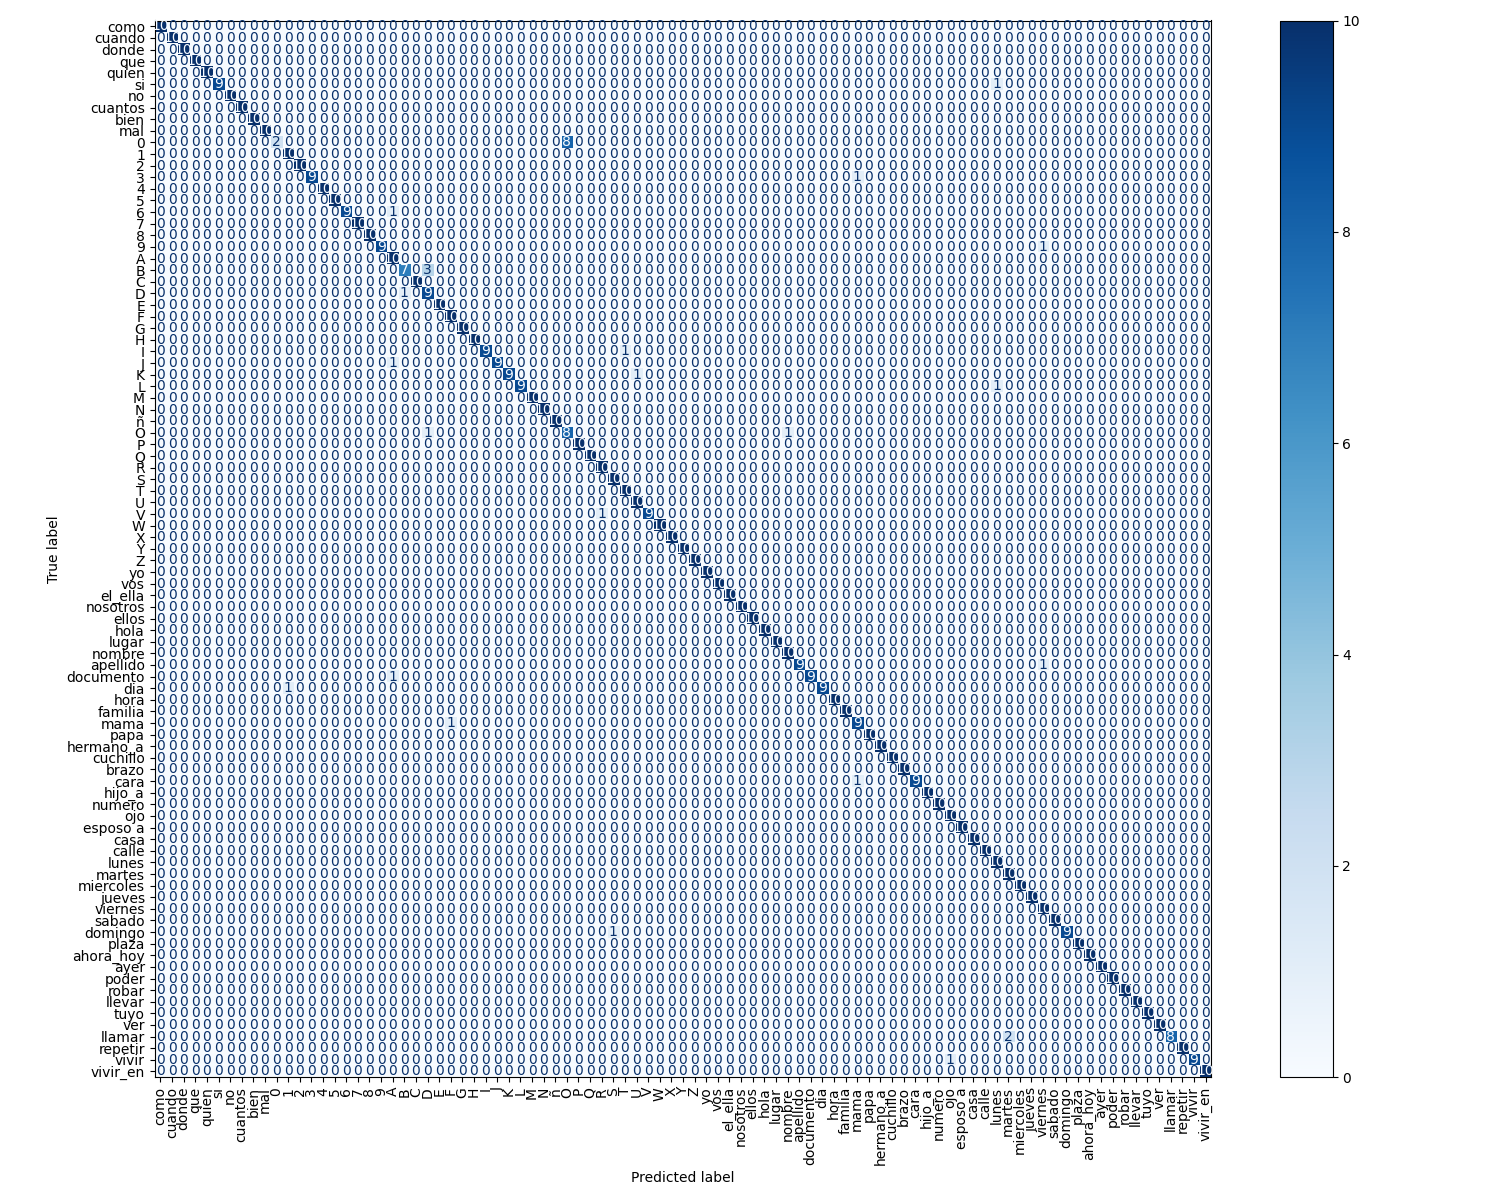
\includegraphics[width=0.72\textwidth]{clasificador/matriz_32_frames_b.png}%
}{%
  \fbox{\parbox{0.72\textwidth}{\centering\vspace{1.5cm}Matriz de confusión del clasificador desplegado\vspace{1.5cm}}}%
}
\caption{Matriz de confusión en validación del clasificador desplegado. Fuente: elaboración propia.}
\label{fig:matriz}
\end{figure}

\chapter{Evaluación}
\section{Cumplimiento de objetivos}
\begin{table}[H]
\centering
\caption{Cumplimiento de objetivos específicos (agosto 2026)}
\label{tab:objetivos}
\begin{tabular}{@{}p{7.2cm}cc@{}}
\toprule
\textbf{Objetivo} & \textbf{Estado} & \textbf{Evidencia} \\
\midrule
Clasificador local de glosas & Cumplido & 91 clases, \texttt{--eval} \\
Traducción semántica integrada & Cumplido (MVP) & \texttt{run.py}, Tabla~\ref{tab:metricas_sem} \\
Segmentación conversacional & Cumplido & \texttt{UtteranceBuffer}, \texttt{RepeatGate} \\
Privacidad / computación en el borde & Cumplido & Sin video a la nube \\
Validación $\geq$80\,\% precisión & Parcial & 90,1\,\% top-3; 71,4\,\% top-1 \\
Avatar y extensión de navegador & Pendiente & Fase final del protocolo \\
\bottomrule
\end{tabular}
\end{table}

\section{Limitaciones}
\begin{itemize}
    \item Brecha entre validación fuera de línea ($\sim$96\,\%) y evaluación con cámara web ($\sim$71\,\% top-1), atribuible a diferencias de dominio entre grabaciones de entrenamiento y uso en vivo.
    \item Conjunto semántico de entrenamiento ($\sim$202 pares) no validado por experta en LSA; evaluación de reserva de un solo turno.
    \item Adaptador LoRA entrenado sin diálogos multi-turno; la memoria conversacional puede desalinear el \textit{prompt} respecto de la distribución de entrenamiento a partir del segundo turno.
    \item Avatar, transcripción del oyente y extensión de navegador pendientes.
    \item Dependencia de encuadre, iluminación y mano dominante (normalización zurdo/diestro parcial).
\end{itemize}

\section{Riesgos detectados}
\begin{itemize}
    \item \textbf{Técnico:} pares de glosas visualmente similares (\texttt{I}/\texttt{T}/\texttt{OJO}) --- mitigado parcialmente por top-3 y contexto del LLM.
    \item \textbf{Datos:} escasez de corpus LSA público --- mitigado con conjunto propio y validación experta.
    \item \textbf{Operativo:} consumo de memoria de video por el LLM --- mitigado con modelo 3B y PEFT; cuantización de 4 bits no activa en la ruta por defecto.
    \item \textbf{Cronograma:} componentes bidireccionales (avatar, extensión) en fase final.
\end{itemize}

\chapter{Conclusiones y trabajos futuros}
\section{Conclusiones}
Se entregó un prototipo funcional de traducción LSA $\rightarrow$ español con procesamiento local. La arquitectura desacoplada por hilos permitió integrar un clasificador compacto, reglas conversacionales propias de la LSA y un traductor semántico sin bloquear la captura de video.

Los resultados muestran que la extracción de puntos corporales es eficiente para inferencia en tiempo pseudo-real, pero la calidad y uniformidad del corpus LSA condicionan el desempeño frente a la cámara más que la complejidad del modelo. La traducción semántica es operativa, aunque las métricas estrictas subestiman traducciones parcialmente correctas. El cumplimiento del objetivo de $\geq$80\,\% de precisión gestual es parcial: alcanzable en top-3, no aún en top-1.

\section{Trabajos futuros}
\begin{itemize}
    \item Validación con personas usuarias sordas en escenarios simulados de emergencia.
    \item Extensión de navegador con superposición de subtítulos y síntesis de voz.
    \item Avatar animado a partir de puntos corporales de referencia (canal Señario).
    \item Captura y procesamiento del turno del oyente (transcripción automática + memoria \texttt{hearing}).
    \item Ampliación y validación experta del corpus semántico; reentrenamiento con diálogos multi-turno.
    \item Reducción de la brecha fuera de línea/en vivo mediante mayor variabilidad en grabaciones y aumento de datos orientado a cámara web.
\end{itemize}

\printbibliography[title={Referencias}]

\appendix
\chapter{Manual de usuario}
Ver \texttt{docs/rama\_integration.md}, sección ``Guía rápida de operación'': teclas \texttt{q} (salir), \texttt{m} (mano dominante), \texttt{c} (captura manual), \texttt{n} (nuevo enunciado).

\chapter{Manual técnico}
\texttt{docs/ficha\_tecnica\_integrador.md} y \texttt{docs/rama\_integration.md} describen arquitectura, configuración, métricas y procedimientos de evaluación.

\chapter{Código fuente}
Repositorio principal (rama \texttt{integration}): \url{https://github.com/FranciscoVeronING/2026_Proyecto_LSA}.\\
Repositorio anterior descartado: \url{https://github.com/FranciscoVeronING/2026---Trabajo-Final-Informatica}.

\chapter{Diagramas completos}
Pendiente: diagrama UML de hilos de trabajo, máquina de estados de \texttt{UtteranceBuffer} y casos de uso CU-01--03 en notación UML.

\chapter{Iteraciones experimentales del clasificador}
\label{anexo:iteraciones}

Antes de seleccionar el \textit{checkpoint} desplegado, se ejecutaron cuatro iteraciones en la rama \texttt{scratch-mediapipe}. La Tabla~\ref{tab:iteraciones} contrasta métricas fuera de línea con evaluación en vivo (\texttt{camera.py --eval}, 91 señas).

\begin{table}[H]
\centering
\caption{Iteraciones experimentales del clasificador}
\label{tab:iteraciones}
\small
\begin{tabular}{@{}clcccc@{}}
\toprule
\textbf{Id} & \textbf{Fotogramas} & \textbf{Arq.} & \textbf{Val acc} & \textbf{Top-1 vivo} & \textbf{Top-3 vivo} \\
\midrule
A & 16 & 128/4h/2L & 97,36\,\% & 61,5\,\% & 83,5\,\% \\
B & 32 & 128/4h/2L & 96,48\,\% & \textbf{71,4\,\%} & 87,9\,\% \\
C & 32 & 64/2h/1L & 97,36\,\% & 67,0\,\% & \textbf{90,1\,\%} \\
D & 32 & Optuna 8 h & 97,69\,\% & 66,0\,\% & 84,6\,\% \\
\bottomrule
\end{tabular}
\end{table}

Se seleccionó la iteración B por mejor top-1 frente a la cámara. Optuna (D) mejoró la pérdida fuera de línea pero no superó B/C en evaluación en vivo.

\begin{figure}[H]
\centering
\IfFileExists{figuras/clasificador/comparativa_iteraciones.png}{%
  \includegraphics[width=\textwidth]{clasificador/comparativa_iteraciones.png}%
}{%
  \fbox{\parbox{\textwidth}{\centering\vspace{1.5cm}Gráfico recomendado: barras top-1/top-3 por iteración (Tabla~\ref{tab:iteraciones})\vspace{1.5cm}}}%
}
\caption{Comparativa de evaluación en vivo por iteración A--D. Fuente: elaboración propia.}
\label{fig:comparativa}
\end{figure}

\chapter{Líneas de trabajo alternativas y cronología del repositorio}
\label{anexo:experimentos}

\section{Ramas del repositorio}
\begin{table}[H]
\centering
\caption{Cronología de ramas en \texttt{2026\_Proyecto\_LSA}}
\label{tab:ramas}
\small
\begin{tabular}{@{}lllp{5cm}@{}}
\toprule
\textbf{Rama} & \textbf{Responsable} & \textbf{Estado} & \textbf{Contenido} \\
\midrule
\texttt{scratch-mediapipe} & Francisco & Entregado & Clasificador desde cero, Optuna \\
\texttt{transfer-mediapipe-*} & Maite & Paralelo & Aprendizaje por transferencia con Keras \\
\texttt{modulo-semantico} & Maite & MVP & Entrenamiento fino LoRA, evaluación BLEU \\
\texttt{integration} & Ambos & Producto final & \texttt{run.py} \\
\texttt{camera\_tests} & Francisco & Archivado & Prototipos tempranos \\
\bottomrule
\end{tabular}
\end{table}

\section{Aprendizaje por transferencia}
Línea con TensorFlow/Keras sobre pesos \texttt{209sontung/sign-language} (\texttt{train\_transfer.py}). Las métricas de validación fueron elevadas en entrenamiento, con menor desempeño en inferencia en vivo respecto de la iteración B entrenada desde cero. También se evaluó SlowFast sobre fotogramas crudos: resultados aceptables pero inferiores en precisión y latencia respecto de puntos corporales.

\section{Corpus ASL descartado}
Los experimentos iniciales con un conjunto ASL evidenciaron sobreajuste y etiquetado inconsistente (dialectos mezclados, videos espejados, oraciones completas etiquetadas como señas aisladas), lo que motivó el corpus LSA propio.

\section{Decisiones técnicas del entrenamiento del clasificador}
Eliminación de malla facial; 32 fotogramas por secuencia; aumento de datos 3D sin espejado; regularización progresiva (\textit{dropout}, suavizado de etiquetas, reducción de capacidad del Transformer); interpolación de fotogramas perdidos; búsqueda con Optuna (8 h).

\chapter{Desarrollo del módulo semántico (MVP)}
\label{anexo:semantico}

Entrega MVP: 24/07/2026. Conjunto \texttt{dataset\_glosas.json} ($\sim$202 pares glosa $\rightarrow$ español, no validado por experta). Entrenamiento fino LoRA con Unsloth; despliegue en \texttt{integration} vía PEFT.

\begin{table}[H]
\centering
\caption{Comparativa de modelos evaluados en \texttt{modulo-semantico}}
\label{tab:llm}
\small
\begin{tabular}{@{}lccc@{}}
\toprule
\textbf{Modelo} & \textbf{BLEU} & \textbf{METEOR} & \textbf{ROUGE-L} \\
\midrule
Qwen 2.5 0.5B & 9,98 & 37,08 & 38,99 \\
Qwen 2.5 1.5B & 19,79 & 49,24 & 52,09 \\
\textbf{Qwen 2.5 3B} & \textbf{48,04} & \textbf{70,87} & \textbf{73,66} \\
Llama 3.2 1B & 19,62 & 45,46 & 47,71 \\
Phi-3-mini-4k & 29,21 & 54,13 & 57,96 \\
\bottomrule
\end{tabular}
\end{table}

\chapter{Figuras recomendadas}
\label{anexo:figuras}
\begin{table}[H]
\centering
\caption{Gráficos complementarios (copiar a \texttt{docs/figuras/})}
\small
\begin{tabular}{@{}llp{5.5cm}@{}}
\toprule
\textbf{Prior.} & \textbf{Archivo} & \textbf{Origen} \\
\midrule
Alta & \texttt{integracion/arquitectura\_pipeline.png} & Diagrama de \texttt{rama\_integration.md} \\
Alta & \texttt{clasificador/matriz\_32\_frames\_b.png} & Iteración B, \texttt{scratch-mediapipe} \\
Alta & \texttt{clasificador/comparativa\_iteraciones.png} & Crear desde Tabla~\ref{tab:iteraciones} \\
Media & \texttt{semantico/barras\_bleu\_modelos.png} & Crear desde Tabla~\ref{tab:llm} \\
Media & \texttt{clasificador/curva\_32\_frames\_b.png} & \texttt{scratch-mediapipe} \\
Baja & \texttt{transfer/accuracy\_lsa.png} & \texttt{transfer-mediapipe-*} \\
\bottomrule
\end{tabular}
\end{table}

\end{document}
